\documentclass[11pt,a4paper]{article}
\usepackage[utf8]{inputenc}
\usepackage[spanish,es-tabla,es-noshorthands]{babel}
\usepackage[margin=2.5cm]{geometry}
\usepackage{booktabs,longtable,array,graphicx,amsmath,xcolor,float,caption,url}
\usepackage{listings}
\usepackage{tikz}
\usetikzlibrary{arrows.meta,positioning,shapes.geometric,fit,calc}
\usepackage[hidelinks]{hyperref}

\newcommand{\aceleracionMedia}{1.05}
\newcommand{\vsGccMedia}{3.1}
\newcommand{\runsPorMedicion}{5}

\newcommand{\vulnTotal}{16}
\newcommand{\vulnPropio}{16}
\newcommand{\vulnEstatico}{10}
\newcommand{\vulnDinamico}{12}
\newcommand{\vulnStackProt}{2}
\newcommand{\vulnAsan}{11}

\newcommand{\fidelidadOk}{199}
\newcommand{\fidelidadTotal}{199}


\newcommand{\cod}[1]{\texttt{#1}}
\lstset{
  basicstyle=\ttfamily\footnotesize, breaklines=true, frame=single, framerule=0.3pt,
  backgroundcolor=\color{black!3}, columns=fullflexible, keepspaces=true, showstringspaces=false,
  xleftmargin=0.5em, xrightmargin=0.5em
}
\captionsetup{font=small}
\setlength{\parskip}{0.4em}
\renewcommand{\arraystretch}{1.1}

\title{Compilador de un subconjunto de C++ a x86-64\\con optimización y seguridad}
\author{Llorent Nunayalle \and Marco Madrid}
\date{Compiladores --- UTEC, ciclo 2026-2\\Proyecto 2, Tipo 2}

\begin{document}
\maketitle

\begin{abstract}
Este reporte describe el diseño, la implementación y la evaluación de un compilador para un subconjunto de C++17
que genera ensamblador x86-64 (GNU as, sintaxis AT\&T, convención System V) ensamblable y enlazable con
herramientas estándar. El compilador incluye análisis léxico, sintáctico y semántico con verificación de tipos y
diagnósticos con ubicación; siete técnicas de optimización activables una a una; y nueve mecanismos de seguridad
(un análisis estático con siete verificaciones y ocho mecanismos dinámicos o de enlace, controlados por banderas). La evaluación experimental, ejecutada
dentro de un contenedor linux/amd64 con \runsPorMedicion{} repeticiones por medición, compara el compilador
con GCC y Clang: las optimizaciones aceleran los benchmarks \aceleracionMedia$\times$ de media geométrica, y los
mecanismos de seguridad detectan \vulnPropio{} de \vulnTotal{} programas con vulnerabilidades intencionales.
\end{abstract}

\tableofcontents
\newpage

%=====================================================================================
\section{Introducción}
\label{sec:intro}
El objetivo del proyecto es construir un compilador completo para un lenguaje existente, respetando sus reglas
léxicas, sintácticas y semánticas, e incorporar optimizaciones y mecanismos de seguridad que prevengan, detecten
o mitiguen errores de memoria y comportamientos indefinidos. El lenguaje elegido es un subconjunto de C++17: un
programa válido del subconjunto debe compilarse y producir exactamente el mismo resultado que con \cod{g++}.

\paragraph{Contribuciones.}
\begin{itemize}
  \item Un frontend completo: scanner, parser descendente recursivo con AST bajo el patrón Visitor y un
        \emph{TypeChecker} que anota el árbol con tipos, símbolos, \emph{layout} y clasificación de la ABI.
  \item Un generador de código x86-64 que implementa clases (constructores, destructor, copia, asignación),
        \cod{const}, referencias, paso y retorno de objetos por valor según System V/Itanium, \cod{new}/\cod{delete},
        arreglos multidimensionales y un runtime propio de \cod{string}, \cod{cout} y \cod{cin}.
  \item Siete optimizaciones (inline, propagación de constantes, plegado y simplificación algebraica, reducción
        de fuerza, eliminación de código muerto e inalcanzable, Sethi-Ullman y optimización de mirilla), cada una
        activable por separado con \cod{--passes}.
  \item Mecanismos de seguridad: análisis estático (siete verificaciones), verificación de límites, de punteros
        nulos, de división entre cero y de desbordamiento aritmético, canarios de pila, asignador instrumentado
        (doble \cod{free}, uso después de liberar, desbordamiento de heap), límite de recursión y endurecimiento
        del binario (PIE, pila no ejecutable, RELRO).
  \item Un conjunto de pruebas (frontend, generación de código, optimización y seguridad), benchmarks, programas
        con vulnerabilidades intencionales y una aplicación web con editor, visualización del AST, del
        ensamblador y de los resultados de optimización y seguridad.
\end{itemize}

\paragraph{Estructura del documento.} La sección~\ref{sec:lenguaje} define el subconjunto; la~\ref{sec:arq}
presenta la arquitectura; la~\ref{sec:front} el frontend; la~\ref{sec:ir} la representación intermedia; la~\ref{sec:opt}
las optimizaciones; la~\ref{sec:seg} la seguridad; la~\ref{sec:gen} la generación de código; la~\ref{sec:eval} la
evaluación experimental y la~\ref{sec:concl} las conclusiones.

%=====================================================================================
\section{Lenguaje seleccionado}
\label{sec:lenguaje}
El lenguaje es C++17 (ISO/IEC 14882:2017, borrador N4659~\cite{cpp17}). La gramática del subconjunto está en
\cod{gramatica.ebnf} (EBNF). Para validar la fidelidad, los resultados esperados de cada prueba se obtienen con
\cod{g++ -std=c++14 -fno-elide-constructors}, que corresponde a la semántica de copia que implementa el compilador
(sin elisión de copias ni constructor de movimiento).

\subsection{Alcance: características incluidas y excluidas}
La tabla~\ref{tab:alcance} resume el alcance y cita las secciones del estándar. Las referencias usan los
identificadores estables del estándar (por ejemplo \cod{[expr.add]}) y el número de cláusula de N4659.

{\footnotesize\raggedright
\begin{longtable}{p{2.6cm}p{4.3cm}p{4.4cm}p{3.4cm}}
\caption{Alcance del subconjunto de C++17.}\label{tab:alcance}\\
\toprule Característica & Estado y justificación & Estándar & Observación \\ \midrule \endfirsthead
\toprule Característica & Estado y justificación & Estándar & Observación \\ \midrule \endhead
Comentarios, identificadores, palabras clave & Incluido: base de cualquier programa & \cod{[lex.comment]} 5.4, \cod{[lex.name]} 5.10, \cod{[lex.key]} 5.11 & Línea y columna en cada token \\
Literales & Incluido: enteros, reales, \cod{char}, cadenas, \cod{true}/\cod{false}, \cod{nullptr} & \cod{[lex.icon]} 5.13.2, \cod{[lex.ccon]} 5.13.3, \cod{[lex.fcon]} 5.13.4, \cod{[lex.string]} 5.13.5, \cod{[lex.nullptr]} 5.13.7 & Sin sufijos (\cod{1.5f}) ni \cod{long long} \\
Tipos fundamentales & Incluido: \cod{int}, \cod{float}, \cod{double}, \cod{bool}, \cod{char}, \cod{void} & \cod{[basic.fundamental]} 6.9.1 & Modelo de datos LP64 \\
Punteros, referencias, arreglos & Incluido: base del lenguaje y de la ABI & \cod{[dcl.ptr]} 11.3.1, \cod{[dcl.ref]} 11.3.2, \cod{[dcl.array]} 11.3.4 & Una dimensión en \cod{new[]} \\
Calificador \cod{const} & Incluido completo: variables, punteros, referencias, métodos & \cod{[dcl.type.cv]} 10.1.7.1, \cod{[conv.qual]} 7.5 & Sin \cod{volatile} ni \cod{mutable} \\
Conversiones estándar & Incluido: promociones, integrales, flotante-entero, booleanas, de puntero & \cod{[conv.prom]} 7.6, \cod{[conv.integral]} 7.8, \cod{[conv.fpint]} 7.10, \cod{[conv.bool]} 7.14 & Sin conversiones definidas por el usuario \\
Operadores & Incluido: aritméticos, relacionales, lógicos con cortocircuito, bit a bit, desplazamientos, asignación, \cod{++}/\cod{--} & \cod{[expr.mul]} 8.6, \cod{[expr.add]} 8.7, \cod{[expr.shift]} 8.8, \cod{[expr.log.and]} 8.14, \cod{[expr.ass]} 8.18 & Sin \cod{?:}, sin asignación compuesta (\cod{+=}) \\
Sentencias de control & Incluido: \cod{if}, \cod{while}, \cod{do}, \cod{for}, \cod{break}, \cod{continue}, \cod{return} & \cod{[stmt.if]} 9.4.1, \cod{[stmt.while]} 9.5.1, \cod{[stmt.for]} 9.5.3, \cod{[stmt.break]} 9.6.1 & Sin \cod{switch} ni \cod{goto} \\
Funciones & Incluido: recursión, parámetros por valor/puntero/referencia, retorno por valor & \cod{[dcl.fct]} 11.3.5, \cod{[basic.start.main]} 6.6.1 & Sin prototipos sin cuerpo, sin sobrecarga, sin argumentos por defecto \\
Clases y \cod{struct} & Incluido: campos, métodos, \cod{this}, \cod{public}/\cod{private} & \cod{[class.mem]} 12.2, \cod{[class.mfct]} 12.2.1, \cod{[class.access]} cláusula 14 & Sin \cod{static}, \cod{friend}, \cod{protected} \\
Constructores y destructor & Incluido: por defecto, con parámetros, de copia, listas de inicialización, inicializadores de campo & \cod{[class.ctor]} 15.1, \cod{[class.dtor]} 15.4, \cod{[class.base.init]} 15.6.2 & Un constructor con parámetros por clase \\
Asignación de copia & Incluido: \cod{T\& operator=(const T\&)} y la implícita & \cod{[class.copy.assign]} 15.8.2, \cod{[over.ass]} 16.5.3 & Es la única sobrecarga de operador \\
Memoria dinámica & Incluido: \cod{new}, \cod{new[]}, \cod{delete}, \cod{delete[]} & \cod{[expr.new]} 8.3.4, \cod{[expr.delete]} 8.3.5 & Sin \cod{placement new} \\
Inicialización & Incluido: directa, de copia, con llaves de agregados & \cod{[dcl.init]} 11.6, \cod{[dcl.init.aggr]} 11.6.1 & Sin listas con \cod{std::initializer\_list} \\
Biblioteca estándar & Incluido lo mínimo: \cod{<iostream>} (\cod{cout}, \cod{cin}, \cod{endl}), \cod{<string>} (métodos básicos), \cod{<cmath>} (\cod{sqrt}) & \cod{[iostream.objects]}, \cod{[string.classes]}, \cod{[c.math]} & El runtime propio no usa libstdc++ \\
Herencia, virtuales, plantillas, excepciones, RTTI, espacios de nombres propios & Excluido: no aportan a los objetivos de optimización y seguridad y multiplican el alcance & cláusulas 13, 17, 18 & Se rechazan con mensaje claro \\
\bottomrule
\end{longtable}
}

\subsection{Diferencias deliberadas respecto a C++17}
\begin{itemize}
  \item No hay constructor ni asignación de movimiento ni elisión de copias: \cod{T t = f();} realiza las dos
        copias de C++14. Por eso los resultados de referencia se obtienen con \cod{-fno-elide-constructors}.
  \item Un literal de cadena se acepta como \cod{char*} (extensión de GCC) además de \cod{const char*}.
  \item Las conversiones implícitas por constructor (\cod{T t = 5;}) se rechazan.
\end{itemize}

%=====================================================================================
\section{Arquitectura del compilador}
\label{sec:arq}
El compilador es un programa C++17 de unas trece mil líneas organizado en módulos acoplados
únicamente por el AST. La figura~\ref{fig:arq} muestra el flujo de compilación.

\begin{figure}[H]
\centering
\begin{tikzpicture}[
  caja/.style={draw, rounded corners, minimum width=2.3cm, minimum height=0.9cm, align=center, font=\small, fill=blue!6},
  opc/.style={draw, rounded corners, minimum width=2.3cm, minimum height=0.9cm, align=center, font=\small, fill=green!8},
  seg/.style={draw, rounded corners, minimum width=2.3cm, minimum height=0.9cm, align=center, font=\small, fill=orange!12},
  flecha/.style={-{Stealth[length=2mm]}, thick}]
  \node[caja] (src) {Código\\fuente};
  \node[caja, right=0.5cm of src] (lex) {Scanner};
  \node[caja, right=0.5cm of lex] (par) {Parser\\(AST)};
  \node[caja, right=0.5cm of par] (tc) {TypeChecker\\(AST anotado)};
  \node[seg, below=0.8cm of tc] (sa) {Análisis estático\\de seguridad};
  \node[opc, left=0.5cm of sa] (op) {Optimizador\\(\cod{-O1})};
  \node[caja, left=0.5cm of op] (gc) {Gencode};
  \node[opc, below=0.8cm of gc] (pp) {Peephole};
  \node[caja, right=0.5cm of pp] (as) {\cod{.s} x86-64};
  \node[seg, right=0.5cm of as] (dyn) {Verificaciones\\dinámicas};
  \node[caja, right=0.5cm of dyn] (bin) {gcc + runtime\\= ejecutable};
  \draw[flecha] (src) -- (lex); \draw[flecha] (lex) -- (par); \draw[flecha] (par) -- (tc);
  \draw[flecha] (tc) -- (sa); \draw[flecha] (sa) -- (op); \draw[flecha] (op) -- (gc);
  \draw[flecha] (gc) -- (pp); \draw[flecha] (pp) -- (as); \draw[flecha, dashed] (gc.south east) to[bend left=15] (dyn.north west);
  \draw[flecha] (as) -- (dyn); \draw[flecha] (dyn) -- (bin);
\end{tikzpicture}
\caption{Flujo de compilación. El optimizador reverifica el AST con el TypeChecker tras cada pase.}
\label{fig:arq}
\end{figure}

\begin{center}
\small
\begin{tabular}{lp{10.2cm}}
\toprule Módulo & Responsabilidad \\ \midrule
\cod{token}, \cod{scanner} & Tokens con línea y columna, comentarios, errores léxicos \\
\cod{ast}, \cod{parser} & Jerarquía de nodos con \cod{accept(Visitor*)}; parser descendente recursivo de 14 niveles de precedencia \\
\cod{type}, \cod{layout} & Modelo de tipos (\cod{constBits}, dimensiones) y estructuras de \emph{layout}/ABI \\
\cod{type\_checker} & Semántica, conversiones, \cod{const}, clases, \emph{layout}, clasificación System V; anota el AST \\
\cod{security\_analysis} & Análisis estático de seguridad con flujo de datos sobre el AST \\
\cod{optimizer}, \cod{peephole} & Siete pases de optimización \\
\cod{gencode} & Visitor que emite ensamblador leyendo solo las anotaciones; verificaciones dinámicas \\
\cod{runtime/runtime.c} & \cod{string}, \cod{cout}, \cod{cin}, asignador instrumentado, \cod{rt\_fail} \\
\cod{api}, \cod{web/} & Modo \cod{--api} (JSON), servidor HTTP y editor web (Docker) \\
\bottomrule
\end{tabular}
\end{center}

\subsection{Uso}
\begin{lstlisting}
./compiler prog.cpp --asm prog.s -O1 --sec=all     # compila con todas las optimizaciones y la seguridad
gcc prog.s runtime/runtime.c -o prog               # ensambla y enlaza (-fPIE -pie ... con --sec=harden)
./compiler prog.cpp -O1 --passes inline,fold --report-opt --asm prog.s
\end{lstlisting}

%=====================================================================================
\section{Frontend}
\label{sec:front}
\subsection{Análisis léxico}
El scanner reconoce palabras clave de C++, identificadores, literales y operadores, descarta comentarios
(\cod{//} y \cod{/* */}) y registra línea y columna de cada token. Los errores léxicos (cadena o carácter sin cerrar,
carácter inválido) se informan con su ubicación. \cod{--scan} lista los tokens.

\subsection{Análisis sintáctico y AST}
El parser es descendente recursivo, con un método por regla de \cod{gramatica.ebnf}. La precedencia de
expresiones se resuelve con una cascada de catorce niveles; el \emph{dangling else} se asocia al \cod{if} más
cercano; \cod{break} y \cod{continue} fuera de un bucle son errores sintácticos. El AST (clases \cod{Exp}, \cod{Stmt}
y declaraciones) usa el patrón Visitor y un identificador \cod{NodeKind} en lugar de RTTI. Cada nodo reserva
campos que las fases posteriores completan (tipo inferido, desplazamientos, función destino, modo de paso de cada
argumento, plan de inicialización de objetos), por lo que el generador no recalcula nada.

\subsection{Análisis semántico y sistema de tipos}
El \emph{TypeChecker} resuelve símbolos con una tabla jerárquica de ámbitos, comprueba tipos y conversiones
implícitas, \cod{const} (un bit por nivel de puntero), referencias (se exige un \emph{lvalue}), acceso
\cod{public}/\cod{private}, constructores disponibles según las reglas de generación implícita de C++, y arma el
\emph{layout} de cada clase (tamaño, alineación y relleno con el modelo LP64). Al terminar, el AST contiene toda
la información que necesita el generador.

\subsection{Manejo de errores}
Se acumulan todos los errores semánticos de un programa. Cada diagnóstico indica fase, mensaje, línea y columna:
\begin{lstlisting}
Error Semantico [Linea 3, Columna 5] Tipo de retorno incompatible en 'suma': se esperaba 'int', pero se devolvio 'int*'
Error Semantico [Linea 5, Columna 20] El miembro 'x' es privado en 'A'
Error Semantico [Linea 9, Columna 16] La declaracion de 'p' requiere el constructor por defecto de 'P', que no existe
\end{lstlisting}
Las pruebas de error (\cod{tests\_gencode/e*.cpp}) verifican 41 mensajes distintos. El editor web subraya el
error en el código fuente.

%=====================================================================================
\section{Representación intermedia}
\label{sec:ir}
\paragraph{Decisión de diseño.}
La representación intermedia de este compilador es el \textbf{AST decorado} que produce el TypeChecker, y no un
código de tres direcciones ni una forma SSA. Todas las optimizaciones y análisis se aplican directamente
sobre esa representación y, para el peephole, sobre el ensamblador generado. La decisión simplifica el
proyecto: el AST ya contiene tipos, símbolos resueltos, desplazamientos, la clasificación de la ABI y el plan de
construcción y destrucción de objetos, que son justamente los datos que una IR de bajo nivel tendría que
reconstruir para soportar clases y paso de objetos por valor.

\paragraph{Construcción.} La IR se construye en dos pasos: el parser crea el AST y el TypeChecker lo anota
(\cod{inferredType}, \cod{VarInfo}, \cod{ArgInfo}, \cod{InitSpec}, \cod{FunctionLayout}). La anotación puede
repetirse sobre el mismo árbol: tras cada pase de optimización se vuelve a ejecutar el TypeChecker, de modo que
ninguna anotación queda obsoleta; si la reverificación falla, el optimizador se descarta y se compila sin optimizar.

\paragraph{Limitaciones.} Al no existir un grafo de flujo de control explícito, los análisis de flujo de datos
(asignación definitiva, hechos sobre punteros) se resuelven sobre la estructura del AST, y no se implementan
optimizaciones que requieren un CFG general (eliminación de subexpresiones comunes global, propagación de
copias entre bloques). Incorporar una IR de tres direcciones con CFG se menciona como trabajo futuro
(sección~\ref{sec:concl}).

%=====================================================================================
\section{Optimización}
\label{sec:opt}
Las optimizaciones solo se ejecutan con \cod{-O1}; \cod{-O0} es el modo por defecto. Cada técnica se activa o
desactiva con \cod{--passes} (por defecto todas) y \cod{--report-opt} lista las transformaciones aplicadas.
Ninguna debe alterar el comportamiento observable: para ello (1) los pases solo reescriben expresiones
\emph{puras} (sin efectos secundarios ni posibilidad de fallo); (2) tras cada pase se reverifica el AST; y
(3) la suite de pruebas compara la salida y el código de retorno de \cod{-O0} y \cod{-O1} sobre
todos los programas de prueba.

\begin{table}[H]
\centering\small
\begin{tabular}{lp{5.3cm}p{5.2cm}}
\toprule Técnica & Descripción & Clasificación \\ \midrule
\cod{inline} & Expansión en línea de funciones pequeñas y puras & Interprocedural (no local) \\
\cod{cprop} & Propagación de constantes & Dentro de la función \\
\cod{fold} & Plegado de constantes y simplificación algebraica & Local \\
\cod{strength} & Reducción de fuerza: \cod{x * 2\textasciicircum{}k} a \cod{x << k} & Local \\
\cod{dce} & Eliminación de código muerto e inalcanzable & Global (por función) \\
\cod{sethi} & Orden de evaluación de Sethi-Ullman & Local (expresiones) \\
\cod{peephole} & Optimización de mirilla sobre el ensamblador & Local (backend) \\
\bottomrule
\end{tabular}
\caption{Técnicas de optimización implementadas.}
\end{table}

\subsection{Análisis de pureza}
\cod{opt::isPure} define cuándo se puede reescribir una expresión: son puros los literales, las lecturas de
variables, la aritmética sin \cod{/} ni \cod{\%} (que pueden fallar) y los campos de objetos nombrados. No son
puros las llamadas, \cod{*p}, \cod{a[i]}, asignaciones, \cod{++}/\cod{--}, \cod{new}/\cod{delete} ni los
\emph{streams}. Por ejemplo \cod{x * 0} pasa a \cod{0} solo si \cod{x} es puro, porque descartarlo omitiría sus
efectos.

\subsection{Plegado de constantes y simplificación algebraica (\cod{fold})}
Evalúa operaciones con operandos literales enteros, booleanos y de carácter, sin tocar los casos que desbordan, la
división entre cero ni los desplazamientos inválidos, y aplica identidades:
\begin{lstlisting}
int x = 2 + 3 * 4;    =>   int x = 14;          // plegado de 3*4 y luego 2+12
y = y + 0;            =>   y = y;               // identidad x + 0
b = false && g();     =>   (no se pliega si g() tuviera efectos)
\end{lstlisting}

\subsection{Propagación de constantes (\cod{cprop})}
Sustituye las lecturas de una variable local que se inicializa con un literal y nunca se modifica después
(sin asignación, \cod{++}/\cod{--}, \cod{\&x}, \cod{cin >> x} ni paso a una referencia), y las constantes
\cod{const} de valor conocido. Después de \cod{cprop} el plegado encuentra más constantes.
\begin{lstlisting}
const int LIM = 6; int n = 10;
for (int i = 0; i < n; i++) ...       =>   for (int i = 0; i < 10; i++) ...
\end{lstlisting}

\subsection{Reducción de fuerza (\cod{strength})}
Reemplaza una multiplicación por una potencia de dos por un desplazamiento (\cod{x * 8} $\rightarrow$
\cod{x << 3}). Como el desplazamiento no detecta el desbordamiento, el pase se desactiva automáticamente con
\cod{--sec=overflow}.

\subsection{Eliminación de código muerto e inalcanzable (\cod{dce})}
Elimina las sentencias que siguen a \cod{return}, \cod{break} o \cod{continue} en el mismo bloque, las ramas
inalcanzables de un \cod{if} con condición constante y los \cod{while} con condición falsa:
\begin{lstlisting}
if (DEBUG) cout << "traza";    // DEBUG vale 0   =>   (eliminado)
return 0;
cout << "nunca";               //                 =>   (eliminado)
\end{lstlisting}

\subsection{Expansión en línea (\cod{inline})}
Solo se expanden funciones libres de una sola sentencia \cod{return expr;}, con tipos escalares, sin llamadas,
variables globales ni \cod{\&\&}/\cod{||}, no recursivas y con argumentos puros del mismo tipo. El cuerpo se clona y
sustituye cada parámetro por su argumento:
\begin{lstlisting}
int sq(int a) { return a * a; }
int y = sq(x);        =>   int y = x * x;       // desaparece "call f_sq"
\end{lstlisting}

\subsection{Sethi-Ullman (\cod{sethi})}
En expresiones enteras puras intercambia los operandos de operadores conmutativos para evaluar primero el
subárbol más pesado (etiqueta de Sethi-Ullman~\cite{sethi70}), con lo que se ahorra un \emph{slot} de pila:
\cod{b + (c * (d + e))} pasa a \cod{((d + e) * c) + b}.

\subsection{Optimización de mirilla (\cod{peephole})}
Opera sobre el ensamblador generado, con ventanas de dos a cuatro instrucciones consecutivas (una etiqueta corta la ventana):
\begin{lstlisting}
leaq -4(%rbp), %rax ; movl (%rax), %eax    =>   movl -4(%rbp), %eax
pushq %rax ; movl $3, %eax ; movl %eax, %ecx ; popq %rax   =>   movl $3, %ecx
pushq %rax ; popq %rax                      =>   (nada)
jmp .L5 ; .L5:                              =>   .L5:
addq $0, %rax                               =>   (nada)
movl %eax, -8(%rbp) ; movl -8(%rbp), %eax   =>   movl %eax, -8(%rbp)
\end{lstlisting}

%=====================================================================================
\section{Seguridad}
\label{sec:seg}
Los mecanismos se seleccionan con \cod{--sec=lista} (\cod{static}, \cod{bounds}, \cod{null}, \cod{div},
\cod{overflow}, \cod{canary}, \cod{heap}, \cod{recursion}, \cod{harden}, o \cod{all}). Los dinámicos pueden
activarse y desactivarse individualmente para medir su costo. Ante una violación, el programa termina de forma
controlada con código de salida 70 y un mensaje con el tipo de error y su ubicación:
\begin{lstlisting}
Error de seguridad: acceso fuera de limites en arreglo en linea 10, columna 10
Error de seguridad: desbordamiento de pila detectado por el canario (funcion declarada en linea 5, columna 5)
\end{lstlisting}

\subsection{Análisis estático (\cod{--sec=static})}
El análisis (\cod{security\_analysis.cpp}) recorre el AST anotado con un estado de flujo de datos (conjunto de
variables definitivamente asignadas y hechos sobre punteros) que se une en las ramas por intersección:
\begin{itemize}
  \item \textbf{Variables sin inicializar}: asignación definitiva sobre \cod{if}, bucles, \cod{break} y
        cortocircuito. Tomar la dirección o pasar la variable por referencia cuenta como asignación.
  \item \textbf{Función sin retorno en todos sus caminos}.
  \item \textbf{Índices fuera de rango conocidos}: índices constantes y bucles
        \cod{for (int i = A; i < B; i++)} con límites constantes cuyo índice llega al tamaño del arreglo.
  \item \textbf{Desbordamiento y división entre cero en expresiones constantes}.
  \item \textbf{Desreferencia de punteros nulos evidentes y uso después de \cod{delete}}, con refinamiento por guardas
        (\cod{if (p)}, \cod{p \&\& *p}).
  \item \textbf{Punteros colgantes} por análisis de tiempo de vida: dirección de una variable local devuelta, y
        puntero que sobrevive al bloque de la variable a la que apunta.
  \item \textbf{Conversiones inseguras}: \cod{double}$\to$\cod{int}, \cod{double}$\to$\cod{float}, constantes que no
        caben en un \cod{char}.
\end{itemize}
Los hallazgos son advertencias con línea y columna. El análisis no produce falsos positivos de estas clases sobre
los 52 programas válidos de las pruebas de generación de código y optimización.

\subsection{Verificaciones dinámicas}
Cada verificación es una comparación en línea con salto a \cod{rt\_fail(tipo, linea, columna)}:
\begin{lstlisting}
# bounds: a[i] sobre un arreglo de 4 elementos
cmpl $4, %eax          # comparacion sin signo: cubre i < 0 e i >= 4
jb   .Lbok3
movl $1, %edi ; movl $10, %esi ; movl $10, %edx
call rt_fail@PLT
.Lbok3:
\end{lstlisting}
\begin{itemize}
  \item \textbf{Límites} (\cod{bounds}): arreglos de tamaño conocido y \cod{string} (\cod{s[i]} válido para $0 \le i \le$ \cod{size()}).
  \item \textbf{Punteros nulos} (\cod{null}): antes de \cod{*p}, \cod{p->campo} y \cod{p[i]}.
  \item \textbf{División entre cero} (\cod{div}) y \textbf{desbordamiento aritmético} (\cod{overflow}):
        \cod{jno} tras \cod{addl}/\cod{subl}/\cod{imull}/\cod{negl}/\cod{++}/\cod{--}, y \cod{INT\_MIN / -1}.
  \item \textbf{Límite de recursión} (\cod{recursion}): contador global incrementado al entrar y decrementado al
        salir de cada función; límite por defecto 20000 (\cod{--max-depth=N}).
\end{itemize}

\subsection{Protección de memoria}
\paragraph{Canario de pila (\cod{canary}).} El TypeChecker reserva \cod{-8(\%rbp)}, por encima de todos los locales.
El prólogo guarda un valor aleatorio por ejecución (\cod{rt\_stack\_guard}, con el byte bajo en cero) y el epílogo lo
compara antes de \cod{leave}; si cambió, se llama a \cod{rt\_fail}.
\begin{lstlisting}
movq rt_stack_guard(%rip), %r11 ; movq %r11, -8(%rbp)     # prologo
...
movq -8(%rbp), %r11 ; cmpq rt_stack_guard(%rip), %r11 ; je .Lok   # epilogo
\end{lstlisting}
\paragraph{Asignador instrumentado (\cod{heap}).} \cod{new}/\cod{delete} usan \cod{rt\_malloc}/\cod{rt\_free}: cada
bloque tiene una cabecera con tamaño y marca y una zona roja de 16 bytes al final. \cod{rt\_free} detecta
doble liberación (marca \emph{FREE}), liberación de punteros ajenos y desbordamiento de heap (zona roja alterada).
Los bloques liberados se rellenan con \cod{0xDD} y pasan a una cuarentena circular de 4096 bloques;
\cod{rt\_check\_ptr} se invoca en cada desreferencia y detecta el uso después de liberar y los punteros nulos.

\subsection{Endurecimiento del binario (\cod{harden})}
El código generado es independiente de la posición (direccionamiento relativo a \cod{\%rip} y llamadas por PLT) y
declara \cod{.note.GNU-stack} (pila no ejecutable). Con \cod{harden} se enlaza con
\cod{-fPIE -pie -Wl,-z,relro,-z,now,-z,noexecstack}; la prueba de seguridad verifica con \cod{readelf} que el
resultado es del tipo DYN, con \cod{GNU\_STACK} sin permiso de ejecución y con \cod{BIND\_NOW}.

%=====================================================================================
\section{Generación de código}
\label{sec:gen}
\subsection{Estructura del ensamblador}
El archivo \cod{.s} contiene una sección \cod{.text} con el código de funciones, métodos, constructores y
destructores; \cod{.bss} con las variables globales (\cod{g\_nombre}, inicializadas por \cod{\_\_init\_globals});
\cod{.rodata} con literales \cod{double} (\cod{.LCn}) y cadenas (\cod{.LSn}); y \cod{.note.GNU-stack}. Los símbolos
codifican su rol: \cod{f\_nombre} (función), \cod{m\_Clase\_metodo}, \cod{ctor\_Clase\_default|args|copy},
\cod{dtor\_Clase}, \cod{assign\_Clase}; \cod{main} es el único símbolo global (\cod{.globl}).

\subsection{Convenciones de llamada}
Se sigue System V AMD64: seis registros enteros (\cod{\%rdi}, \cod{\%rsi}, \cod{\%rdx}, \cod{\%rcx}, \cod{\%r8}, \cod{\%r9}),
ocho registros SSE y el resto en la pila, con \cod{\%rsp} alineado a 16 antes de cada \cod{call}. Los argumentos se
evalúan a temporales y después se cargan en registros, de modo que una llamada anidada no los destruya. Los
objetos pequeños triviales se reparten por \emph{eightbytes} (clase INTEGER o SSE); los no triviales
(constructor de copia o destructor propio, o con \cod{string}) se pasan por referencia invisible y se devuelven por
puntero oculto, siguiendo las reglas de Itanium. La clasificación (\cod{classifyRecord}, \cod{computeAbi}) la
calcula el TypeChecker.

\subsection{Marco de pila y manejo de memoria}
Cada función usa \cod{pushq \%rbp; movq \%rsp,\%rbp; subq \$N,\%rsp} con \cod{N} múltiplo de 16 y copia los parámetros a su
\emph{slot}. Los resultados de expresiones viajan en \cod{\%eax}, \cod{\%rax} o \cod{\%xmm0} según el tipo. El ciclo de vida
de los objetos se gestiona con pilas de scopes y temporales: los destructores se ejecutan al salir de cada bloque,
en \cod{return}, \cod{break}, \cod{continue}, con \cod{delete}, al final de la expresión completa para los temporales y,
para los globales, en orden inverso en \cod{\_\_fini\_globals}.

\subsection{Runtime}
\cod{runtime/runtime.c} implementa \cod{string} dinámico (copia profunda, crecimiento por duplicación), \cod{cout}/\cod{cin} y,
para la seguridad, el asignador instrumentado, \cod{rt\_stack\_guard}, \cod{rt\_depth} y \cod{rt\_fail}.

%=====================================================================================
\section{Evaluación experimental}
\label{sec:eval}
\subsection{Metodología y entorno}
Todas las mediciones se ejecutan dentro de un contenedor Docker linux/amd64 (imagen \cod{mc-bench}: GCC 13.5 y
Clang 14), donde también se compila el compilador propio, para que los tiempos de compilación sean comparables.
Cada medición se repite \runsPorMedicion{} veces más una de calentamiento; se reportan media, desviación estándar
muestral e intervalo de confianza del 95\,\% (distribución $t$). Todas las salidas de los programas se comparan con
la de \cod{g++ -O0}: \fidelidadOk{} de \fidelidadTotal{} binarios producen exactamente la misma salida.

\begin{table}[H]
\centering\small
\begin{tabular}{ll}\toprule
Elemento & Valor \\\midrule
Arquitectura & x86\_64 \\
Sistema & Linux-6.12.76-linuxkit-x86\_64-with-glibc2.36 \\
CPU & VirtualApple @ 2.50GHz \\
Compilador de referencia 1 & gcc (GCC) 13.5.0 \\
Compilador de referencia 2 & Debian clang version 14.0.6 \\
Ensamblador & GNU assembler (GNU Binutils for Debian) 2.40 \\
Ejecuciones por medicion & 5 (mas una de calentamiento) \\
\bottomrule\end{tabular}

\caption{Entorno experimental.}
\end{table}

\paragraph{Benchmarks.} Ocho programas del subconjunto (\cod{benchmarks/}): recursión (\cod{fib}), criba de
Eratóstenes, producto de matrices de \cod{double}, conteo de primos por división, integración de un oscilador,
objetos (constructores, destructor, copia por valor), ordenamiento burbuja y memoria dinámica con \cod{string}.

\subsection{Fidelidad al lenguaje}
Además de los benchmarks, la suite del compilador compara la salida contra \cod{g++} en 84 programas de generación
de código (incluidos 41 casos de error de compilación), 9 del frontend y 57 de optimización (cada uno con \cod{-O0} y
\cod{-O1}); todos pasan, también con \cod{--sec=all} y con AddressSanitizer sobre el ejecutable.

\subsection{Rendimiento}
\begin{table}[H]
\centering\scriptsize
\resizebox{\textwidth}{!}{\begin{tabular}{lrrrrrrrr}\toprule
Programa & gcc -O0 & gcc -O2 & clang -O0 & clang -O2 & propio -O0 & propio -O1 & Aceleracion -O1/-O0 & -O1 / gcc -O2 \\\midrule
fib & 302 $\pm$ 46 & 99 $\pm$ 19 & 285 $\pm$ 5 & 184 $\pm$ 12 & 460 $\pm$ 25 & 355 $\pm$ 5 & 1.30$\times$ & 3.6$\times$ \\
criba & 303 $\pm$ 45 & 282 $\pm$ 41 & 212 $\pm$ 40 & 281 $\pm$ 24 & 361 $\pm$ 22 & 429 $\pm$ 100 & 0.84$\times$ & 1.5$\times$ \\
matmul & 131 $\pm$ 3 & 123 $\pm$ 14 & 162 $\pm$ 9 & 55 $\pm$ 3 & 369 $\pm$ 38 & 669 $\pm$ 114 & 0.55$\times$ & 5.4$\times$ \\
primos & 154 $\pm$ 3 & 137 $\pm$ 7 & 161 $\pm$ 7 & 117 $\pm$ 13 & 460 $\pm$ 64 & 478 $\pm$ 108 & 0.96$\times$ & 3.5$\times$ \\
oscilador & 561 $\pm$ 43 & 197 $\pm$ 12 & 570 $\pm$ 70 & 205 $\pm$ 11 & 1047 $\pm$ 92 & 1053 $\pm$ 116 & 0.99$\times$ & 5.3$\times$ \\
vectores & 501 $\pm$ 34 & 119 $\pm$ 2 & 755 $\pm$ 193 & 123 $\pm$ 5 & 1009 $\pm$ 213 & 767 $\pm$ 50 & 1.31$\times$ & 6.4$\times$ \\
burbuja & 79 $\pm$ 0 & 178 $\pm$ 10 & 108 $\pm$ 3 & 49 $\pm$ 0 & 325 $\pm$ 10 & 218 $\pm$ 1 & 1.49$\times$ & 1.2$\times$ \\
memoria & 263 $\pm$ 9 & 234 $\pm$ 6 & 347 $\pm$ 46 & 208 $\pm$ 8 & 596 $\pm$ 53 & 469 $\pm$ 24 & 1.27$\times$ & 2.0$\times$ \\
\midrule
Media geometrica &  &  &  &  &  &  & 1.05$\times$ & 3.1$\times$ \\
\bottomrule\end{tabular}
}
\caption{Tiempo de ejecución en ms (media $\pm$ desviación estándar).}
\label{tab:rend}
\end{table}
\begin{figure}[H]
\centering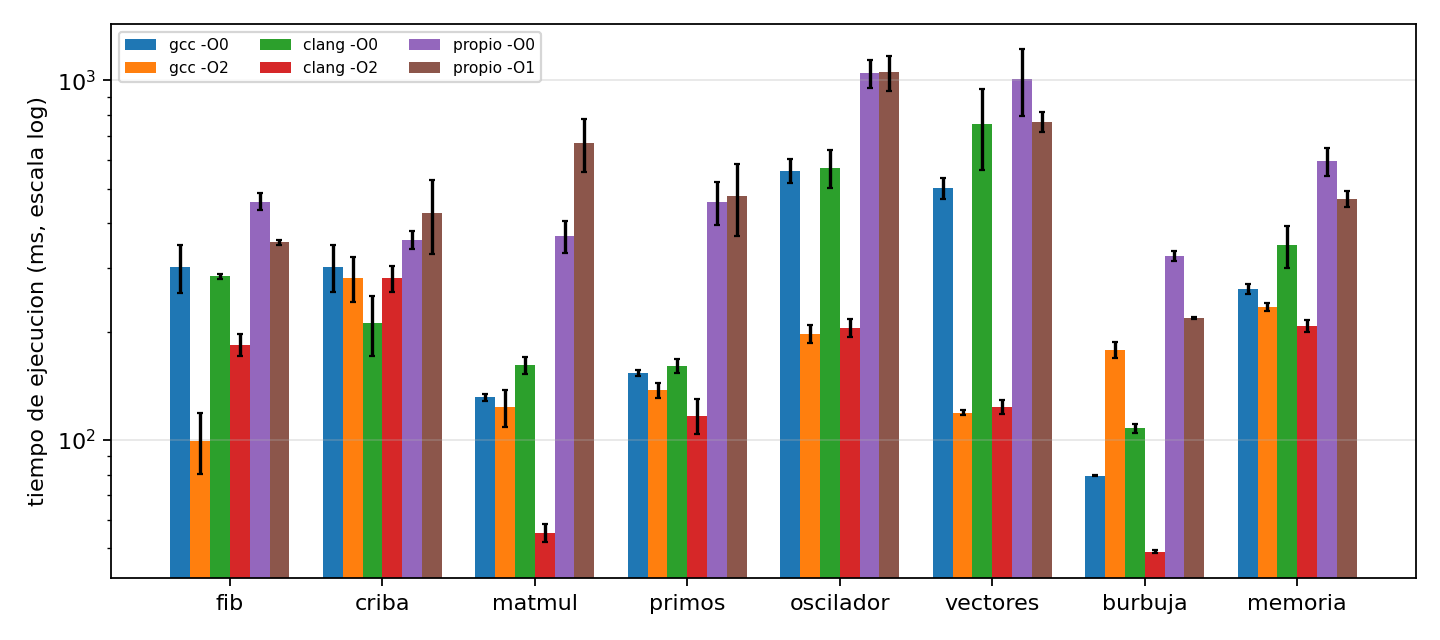
\includegraphics[width=0.95\textwidth]{figuras/tiempos.png}
\caption{Tiempo de ejecución por configuración (escala logarítmica, barras de error: desviación estándar).}
\end{figure}
Con \cod{-O1}, el compilador acelera los benchmarks \aceleracionMedia$\times$ (media geométrica) respecto de su
\cod{-O0}. Frente a \cod{gcc -O2}, el código generado es \vsGccMedia$\times$ más lento en media geométrica: es el
orden de magnitud esperable de un generador que mantiene los temporales en pila y no asigna registros a variables.

\subsection{Calidad del código}
\begin{table}[H]
\centering\small
\resizebox{\textwidth}{!}{\begin{tabular}{lrrrrr}\toprule
Configuracion & Instrucciones & Bytes de .text & Tamano del ejecutable (KB) & Compilacion (ms) & Tiempo ejec. (ms) \\\midrule
gcc -O0 & 117 & 415 & 16.2 & 627.4 & 240 \\
gcc -O2 & 149 & 551 & 16.0 & 846.2 & 162 \\
clang -O0 & 127 & 514 & 16.5 & 1128.1 & 266 \\
clang -O2 & 146 & 564 & 16.4 & 1554.0 & 131 \\
propio -O0 & 238 & 699 & 22.4 & 103.8 & 525 \\
propio -O1 & 196 & 611 & 22.4 & 110.1 & 502 \\
\bottomrule\end{tabular}
}
\caption{Promedio sobre los benchmarks: instrucciones del objeto, bytes de \cod{.text}, tamaño del ejecutable y
tiempo de compilación (compilador propio: compilador + ensamblado; gcc/clang: \cod{-c}).}
\end{table}
El tiempo de compilación del compilador propio es menor porque no analiza las cabeceras de la biblioteca estándar.

\subsection{Impacto de cada optimización}
\begin{table}[H]
\centering\small
\resizebox{\textwidth}{!}{\begin{tabular}{lrrr}\toprule
Pase & Aceleracion (media geom.) & Mejor caso & Instrucciones (\%) \\\midrule
inline & 0.958$\times$ & 1.16$\times$ & +0.0 \\
cprop & 0.948$\times$ & 1.25$\times$ & -0.6 \\
fold & 0.912$\times$ & 1.21$\times$ & +0.0 \\
strength & 0.908$\times$ & 1.23$\times$ & +0.0 \\
dce & 0.931$\times$ & 1.16$\times$ & +0.0 \\
sethi & 0.937$\times$ & 1.21$\times$ & +0.0 \\
peephole & 1.169$\times$ & 1.50$\times$ & -16.9 \\
\midrule
Todos (-O1) & 1.05$\times$ & 1.49$\times$ & -17.2 \\
\bottomrule\end{tabular}
}
\caption{Impacto individual de cada pase aplicado solo frente a \cod{-O0}. Media geométrica sobre los benchmarks.}
\end{table}
\begin{figure}[H]
\centering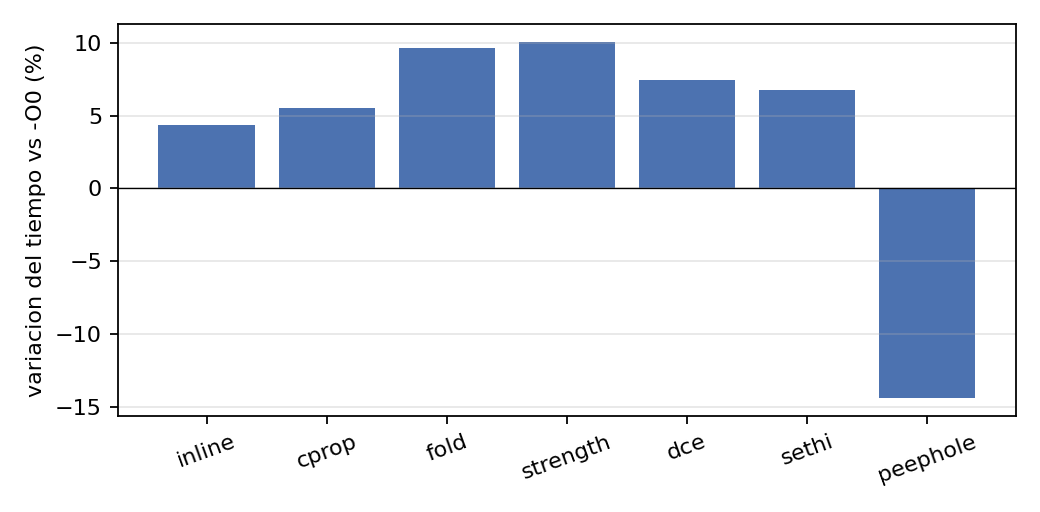
\includegraphics[width=0.75\textwidth]{figuras/impacto_pases.png}
\caption{Variación del tiempo de ejecución por pase frente a \cod{-O0} (negativa: más rápido).}
\end{figure}
Con \cod{-O1} la aceleración global es modesta (\aceleracionMedia$\times$), y casi toda procede de \cod{peephole}, que
elimina cerca de una sexta parte de las instrucciones. Los demás pases (\cod{inline}, \cod{cprop}, \cod{fold},
\cod{strength}, \cod{dce}, \cod{sethi}) transforman patrones concretos que casi no aparecen en estos benchmarks, y
con \runsPorMedicion{} repeticiones sus diferencias de tiempo (alrededor de $\pm 10$\,\%) quedan dentro del ruido
de medición del entorno; el efecto verificable de cada uno es la reducción de instrucciones y las transformaciones
que informa \cod{--report-opt}. El apéndice~\ref{ap:tablas} lista los tiempos
completos por programa.

\subsection{Efectividad de la seguridad}
Se escribieron \vulnTotal{} programas con vulnerabilidades intencionales (\cod{vulnerabilidades/}) y se ejecutaron
con el compilador propio y con los mecanismos equivalentes de GCC y Clang. La tabla~\ref{tab:efect} usa:
\textbf{S} aviso del análisis estático; \textbf{D} terminación con diagnóstico específico; \textbf{C} terminación
anormal sin diagnóstico (por ejemplo, una señal); \textbf{W} advertencia de \cod{-Wall -Wextra}; -- no detectado.

\begin{table}[H]
\centering\scriptsize
\resizebox{\textwidth}{!}{\begin{tabular}{llcccccccc}\toprule
 & & \multicolumn{3}{c}{Este compilador} & \multicolumn{2}{c}{gcc} & \multicolumn{2}{c}{clang} & gcc \\
\cmidrule(lr){3-5}\cmidrule(lr){6-7}\cmidrule(lr){8-9}
Programa & Vulnerabilidad & estatico & dinamico (mecanismo) & todos & stack-prot & asan+ubsan & asan+ubsan & -Wall \\\midrule
v01 & desbordamiento de pila & S & bounds, canary & D & D & D & D & -- \\
v02 & indice constante fuera de rango & S & bounds & D & -- & D & D & -- \\
v03 & puntero nulo evidente & S & null, heap & D & C & D & D & -- \\
v04 & puntero nulo dinamico & -- & null, heap & D & C & D & D & -- \\
v05 & division entre cero & -- & div & D & C & D & D & -- \\
v06 & desbordamiento de entero & -- & overflow & D & -- & D & D & -- \\
v07 & desbordamiento constante & S & div, overflow & D & C & D & D & W \\
v08 & uso despues de liberar & S & heap & D & -- & D & D & -- \\
v09 & doble liberacion & S & -- & D & D & D & D & -- \\
v10 & variable sin inicializar & S & -- & -- & -- & -- & -- & -- \\
v11 & retorno faltante & S & -- & -- & -- & -- & -- & -- \\
v12 & recursion infinita & -- & recursion & D & C & D & D & -- \\
v13 & puntero colgante & S & -- & -- & -- & -- & -- & W \\
v14 & desbordamiento de heap & -- & heap & D & -- & D & D & -- \\
v15 & indice de string & -- & bounds & D & -- & -- & -- & -- \\
v16 & conversion insegura & S & -- & -- & -- & -- & -- & W \\
\midrule
Detectadas & & 10/16 & 11/16 & 12/16 & 2/16 & 11/16 & 11/16 & 3/16 \\
\bottomrule\end{tabular}
}
\caption{Detección de vulnerabilidades. La doble liberación también la detecta glibc sin ninguna protección.}
\label{tab:efect}
\end{table}
\begin{figure}[H]
\centering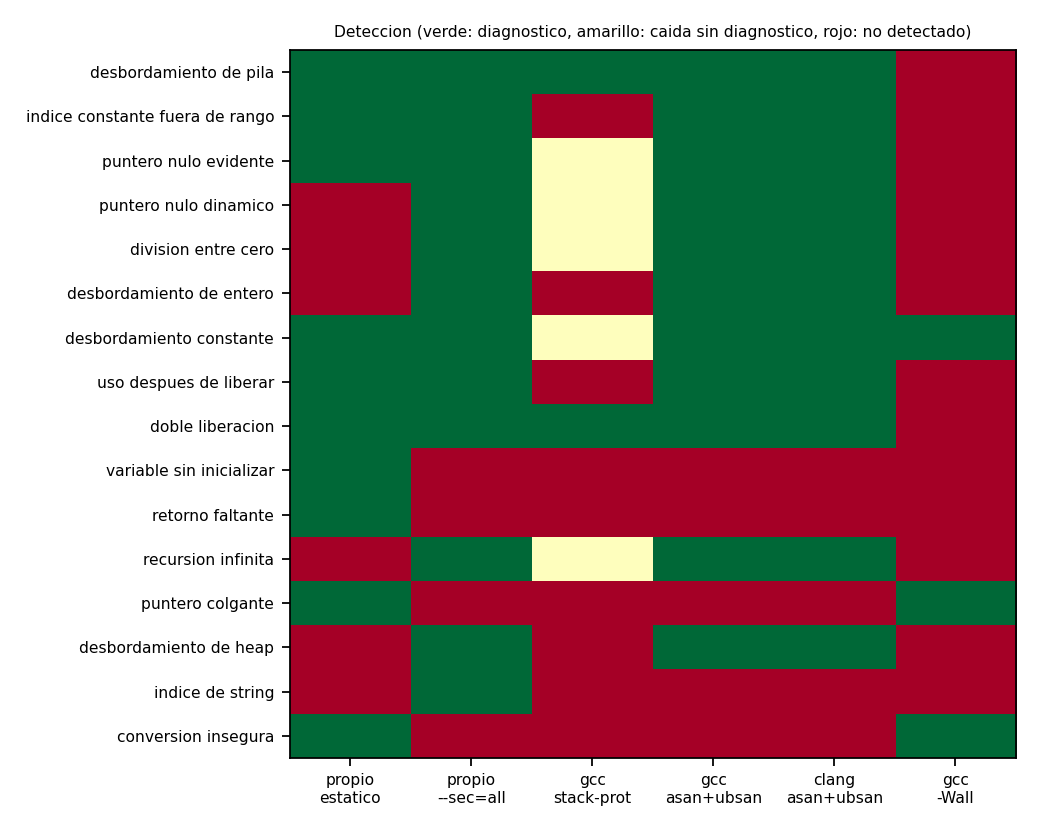
\includegraphics[width=0.7\textwidth]{figuras/efectividad.png}
\caption{Mapa de detección por mecanismo.}
\end{figure}
Con todos los mecanismos, el compilador propio detecta \vulnPropio{} de \vulnTotal{} programas (\vulnEstatico{} por el
análisis estático y \vulnDinamico{} en ejecución); GCC con \cod{-fstack-protector-all} detecta \vulnStackProt{} y con
\cod{-fsanitize=address,undefined}, \vulnAsan{}. El análisis estático complementa a los sanitizers en las
vulnerabilidades que no dependen de la ejecución (variable sin inicializar, retorno faltante, puntero colgante), que
los sanitizers de ejecución no ven, y los sanitizers no detectan el índice fuera de rango dentro de un \cod{std::string}
que sí detecta la verificación de límites propia.

\subsection{Costo de la seguridad}
\begin{table}[H]
\centering\small
\resizebox{\textwidth}{!}{\begin{tabular}{lrrrr}\toprule
Mecanismo & Sobrecarga media (\%) & Peor caso (\%) & Instrucciones (\%) & .text (\%) \\\midrule
bounds & +6.3 & +36.6 & +8.1 & +12.6 \\
null & +4.0 & +21.2 & +0.7 & +1.1 \\
div & +8.3 & +41.5 & +3.6 & +5.5 \\
overflow & +13.6 & +70.6 & +21.6 & +33.2 \\
canary & +0.6 & +41.8 & +9.5 & +16.4 \\
heap & +2.3 & +21.3 & +0.0 & +0.0 \\
recursion & +8.2 & +38.3 & +8.4 & +16.4 \\
harden & +9.4 & +63.3 & +0.0 & +0.0 \\
todos (--sec=all) & +77.1 & +3774.3 & +52.4 & +85.7 \\
\midrule
todos con -O1 (vs -O1) & +75.5 & +4925.0 & -- & -- \\
\bottomrule\end{tabular}
}
\caption{Sobrecarga de cada mecanismo frente al mismo compilador con \cod{-O0} (media geométrica sobre los benchmarks).}
\end{table}
\begin{table}[H]
\centering\small
\begin{tabular}{lrr}\toprule
Referencia (vs gcc -O0) & Sobrecarga media (\%) & Peor caso (\%) \\\midrule
gcc -fstack-protector-all & +13.0 & +53.0 \\
gcc -fsanitize=address,undefined & +188.3 & +869.5 \\
\bottomrule\end{tabular}

\caption{Sobrecarga de los mecanismos equivalentes de gcc y clang frente a \cod{-O0} sin protección.}
\end{table}
\begin{figure}[H]
\centering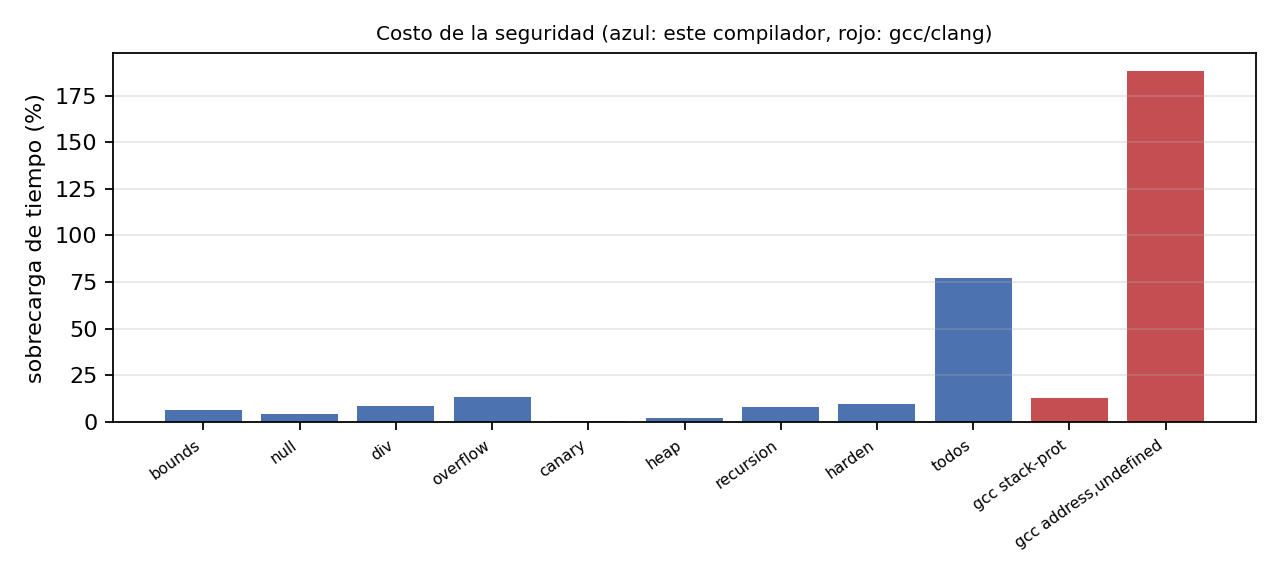
\includegraphics[width=0.85\textwidth]{figuras/costo_seguridad.png}
\caption{Sobrecarga de ejecución de cada mecanismo.}
\end{figure}

\subsection{Amenazas a la validez}
\begin{itemize}
  \item Los tiempos se midieron en un contenedor amd64 ejecutado sobre un procesador Apple mediante traducción
        binaria; las comparaciones relativas dentro del mismo entorno son válidas, pero los valores absolutos
        no son extrapolables a hardware x86 nativo.
  \item Los benchmarks son programas cortos del subconjunto; el rendimiento frente a GCC/Clang en programas
        mayores puede diferir.
  \item El tiempo de compilación de gcc y clang incluye el análisis de \cod{<iostream>}; el del compilador propio no.
  \item La medición de \cod{--sec=heap} sobre el benchmark de memoria con la primera versión de la cuarentena (4096 bloques,
        búsqueda lineal en cada acceso) no terminó en un tiempo razonable y se descartó; la cuarentena se redujo a 64
        bloques con filtro por rango de direcciones. Aun así, \cod{--sec=all} multiplica el tiempo de ese benchmark
        por su verificación en cada acceso a memoria dinámica.
  \item La efectividad se mide con dieciséis programas diseñados para el estudio; no es una cobertura exhaustiva
        de clases de vulnerabilidades.
\end{itemize}

%=====================================================================================
\section{Conclusiones}
\label{sec:concl}
Se construyó un compilador de un subconjunto de C++17 a x86-64 con frontend completo, generación de código que
respeta la ABI System V, siete optimizaciones activables por separado y nueve mecanismos de seguridad, con una
suite de pruebas que verifica la fidelidad frente a \cod{g++} y la ausencia de regresiones al activar
optimizaciones o seguridad. Las mediciones muestran que las optimizaciones reducen el tiempo de ejecución y que
los mecanismos de seguridad detectan la mayoría de las vulnerabilidades intencionales con un costo medible y
configurable.

\paragraph{Limitaciones y trabajo futuro.}
\begin{itemize}
  \item La representación intermedia es el AST decorado; una IR de tres direcciones con grafo de flujo de control
        permitiría eliminación global de subexpresiones, propagación de copias, motion de código invariante y
        asignación de registros, y reduciría la brecha frente a \cod{gcc -O2}.
  \item Herencia, funciones virtuales, plantillas y excepciones quedan fuera del subconjunto.
  \item No hay pila sombra ni integridad completa del flujo de control; la verificación de límites de punteros
        arbitrarios requiere metadatos de tamaño (el asignador instrumentado cubre el heap).
\end{itemize}

\paragraph{Declaración de uso de herramientas de inteligencia artificial.}
Durante el desarrollo se usó un asistente de IA (Claude Code) como apoyo complementario para la implementación
de pases, pruebas, scripts de experimentación y redacción. Las decisiones de diseño, el alcance del subconjunto
y la interpretación de los resultados fueron revisados por los integrantes del grupo.

%=====================================================================================
\begin{thebibliography}{99}
\bibitem{cpp17} ISO/IEC 14882:2017. \emph{Programming Languages --- C++}. Borrador de trabajo N4659.
\bibitem{sysv} M. Matz, J. Hubi\v{c}ka, A. Jaeger, M. Mitchell. \emph{System V Application Binary Interface, AMD64 Architecture Processor Supplement}.
\bibitem{itanium} \emph{Itanium C++ ABI}. \url{https://itanium-cxx-abi.github.io/cxx-abi/abi.html}.
\bibitem{aho} A. Aho, M. Lam, R. Sethi, J. Ullman. \emph{Compilers: Principles, Techniques, and Tools}, 2.\textsuperscript{a} ed. Pearson, 2006.
\bibitem{muchnick} S. Muchnick. \emph{Advanced Compiler Design and Implementation}. Morgan Kaufmann, 1997.
\bibitem{cooper} K. Cooper, L. Torczon. \emph{Engineering a Compiler}, 2.\textsuperscript{a} ed. Morgan Kaufmann, 2011.
\bibitem{sethi70} R. Sethi, J. Ullman. The generation of optimal code for arithmetic expressions. \emph{J. ACM} 17(4), 1970.
\bibitem{stackguard} C. Cowan et al. StackGuard: automatic adaptive detection and prevention of buffer-overflow attacks. \emph{USENIX Security}, 1998.
\bibitem{asan} K. Serebryany, D. Bruening, A. Potapenko, D. Vyukov. AddressSanitizer: a fast address sanity checker. \emph{USENIX ATC}, 2012.
\bibitem{gas} \emph{Using as}, the GNU assembler. Free Software Foundation.
\bibitem{gccopts} \emph{GCC Command Options}: \cod{-fstack-protector}, \cod{-fsanitize}. \url{https://gcc.gnu.org/onlinedocs/gcc/}.
\end{thebibliography}

\appendix
\section{Tablas completas}
\label{ap:tablas}
\begin{table}[H]
\centering\scriptsize
\resizebox{\textwidth}{!}{\begin{tabular}{lrrrrrrrrr}\toprule
Programa & O0 & O1 & only\_inline & only\_cprop & only\_fold & only\_strength & only\_dce & only\_sethi & only\_peephole \\\midrule
fib & 460 & 355 & 511 & 465 & 479 & 641 & 507 & 583 & 478 \\
criba & 361 & 429 & 362 & 501 & 355 & 510 & 375 & 412 & 319 \\
matmul & 369 & 669 & 559 & 446 & 616 & 480 & 414 & 371 & 367 \\
primos & 460 & 478 & 397 & 415 & 599 & 441 & 515 & 508 & 341 \\
oscilador & 1047 & 1053 & 1029 & 1193 & 1220 & 1183 & 1028 & 993 & 1149 \\
vectores & 1009 & 767 & 871 & 806 & 835 & 823 & 870 & 836 & 727 \\
burbuja & 325 & 218 & 371 & 384 & 314 & 330 & 364 & 337 & 216 \\
memoria & 596 & 469 & 590 & 556 & 599 & 559 & 776 & 769 & 479 \\
\bottomrule\end{tabular}
}
\caption{Tiempo medio (ms) de cada pase aplicado solo.}
\end{table}
\begin{table}[H]
\centering\scriptsize
\resizebox{\textwidth}{!}{\begin{tabular}{lrrrrrrrrrr}\toprule
Programa & O0 & bounds & null & div & overflow & canary & heap & recursion & harden & all \\\midrule
fib & 460 & 629 & 536 & 651 & 528 & 618 & 558 & 636 & 545 & 674 \\
criba & 361 & 392 & 437 & 492 & 615 & 511 & 373 & 397 & 390 & 412 \\
matmul & 369 & 318 & 298 & 378 & 316 & 273 & 356 & 271 & 459 & 308 \\
primos & 460 & 401 & 487 & 414 & 557 & 402 & 487 & 491 & 423 & 515 \\
oscilador & 1047 & 1234 & 1105 & 1106 & 1239 & 1125 & 1162 & 1258 & 1050 & 1089 \\
vectores & 1009 & 874 & 927 & 963 & 966 & 954 & 876 & 967 & 806 & 1142 \\
burbuja & 325 & 373 & 343 & 345 & 383 & 310 & 308 & 335 & 347 & 439 \\
memoria & 596 & 742 & 660 & 594 & 610 & 525 & -- & 787 & 973 & 23077 \\
\bottomrule\end{tabular}
}
\caption{Tiempo medio (ms) con cada mecanismo de seguridad.}
\end{table}

\section{Repositorio y reproducción}
Repositorio público del proyecto: \url{https://github.com/MarcoMadridG27/proyecto-compi}

Aplicación web (editor, AST, ensamblador, optimizaciones): \url{https://compilador.marcomadrid.dev}

El código, las pruebas, los benchmarks y los programas con vulnerabilidades están en el repositorio. Para repetir
los experimentos y regenerar este reporte:
\begin{lstlisting}
make                                              # compila el compilador
python3 run_tests.py && python3 run_gencode_tests.py && python3 run_opt_tests.py && python3 run_security_tests.py
benchmarks/ejecutar_experimentos.sh todo 10       # mide (docker, linux/amd64)
python3 documentacion/reporte/generar_datos.py    # tablas y figuras
documentacion/reporte/compilar.sh                 # genera reporte.pdf
\end{lstlisting}

\end{document}
